\documentclass{article} % For LaTeX2e
\usepackage{iclr2021_conference,times}

% Optional math commands from https://github.com/goodfeli/dlbook_notation.
%%%%% NEW MATH DEFINITIONS %%%%%

\usepackage{amsmath,amsfonts,bm}

% Mark sections of captions for referring to divisions of figures
\newcommand{\figleft}{{\em (Left)}}
\newcommand{\figcenter}{{\em (Center)}}
\newcommand{\figright}{{\em (Right)}}
\newcommand{\figtop}{{\em (Top)}}
\newcommand{\figbottom}{{\em (Bottom)}}
\newcommand{\captiona}{{\em (a)}}
\newcommand{\captionb}{{\em (b)}}
\newcommand{\captionc}{{\em (c)}}
\newcommand{\captiond}{{\em (d)}}

% Highlight a newly defined term
\newcommand{\newterm}[1]{{\bf #1}}


% Figure reference, lower-case.
\def\figref#1{figure~\ref{#1}}
% Figure reference, capital. For start of sentence
\def\Figref#1{Figure~\ref{#1}}
\def\twofigref#1#2{figures \ref{#1} and \ref{#2}}
\def\quadfigref#1#2#3#4{figures \ref{#1}, \ref{#2}, \ref{#3} and \ref{#4}}
% Section reference, lower-case.
\def\secref#1{section~\ref{#1}}
% Section reference, capital.
\def\Secref#1{Section~\ref{#1}}
% Reference to two sections.
\def\twosecrefs#1#2{sections \ref{#1} and \ref{#2}}
% Reference to three sections.
\def\secrefs#1#2#3{sections \ref{#1}, \ref{#2} and \ref{#3}}
% Reference to an equation, lower-case.
\def\eqref#1{equation~\ref{#1}}
% Reference to an equation, upper case
\def\Eqref#1{Equation~\ref{#1}}
% A raw reference to an equation---avoid using if possible
\def\plaineqref#1{\ref{#1}}
% Reference to a chapter, lower-case.
\def\chapref#1{chapter~\ref{#1}}
% Reference to an equation, upper case.
\def\Chapref#1{Chapter~\ref{#1}}
% Reference to a range of chapters
\def\rangechapref#1#2{chapters\ref{#1}--\ref{#2}}
% Reference to an algorithm, lower-case.
\def\algref#1{algorithm~\ref{#1}}
% Reference to an algorithm, upper case.
\def\Algref#1{Algorithm~\ref{#1}}
\def\twoalgref#1#2{algorithms \ref{#1} and \ref{#2}}
\def\Twoalgref#1#2{Algorithms \ref{#1} and \ref{#2}}
% Reference to a part, lower case
\def\partref#1{part~\ref{#1}}
% Reference to a part, upper case
\def\Partref#1{Part~\ref{#1}}
\def\twopartref#1#2{parts \ref{#1} and \ref{#2}}

\def\ceil#1{\lceil #1 \rceil}
\def\floor#1{\lfloor #1 \rfloor}
\def\1{\bm{1}}
\newcommand{\train}{\mathcal{D}}
\newcommand{\valid}{\mathcal{D_{\mathrm{valid}}}}
\newcommand{\test}{\mathcal{D_{\mathrm{test}}}}

\def\eps{{\epsilon}}


% Random variables
\def\reta{{\textnormal{$\eta$}}}
\def\ra{{\textnormal{a}}}
\def\rb{{\textnormal{b}}}
\def\rc{{\textnormal{c}}}
\def\rd{{\textnormal{d}}}
\def\re{{\textnormal{e}}}
\def\rf{{\textnormal{f}}}
\def\rg{{\textnormal{g}}}
\def\rh{{\textnormal{h}}}
\def\ri{{\textnormal{i}}}
\def\rj{{\textnormal{j}}}
\def\rk{{\textnormal{k}}}
\def\rl{{\textnormal{l}}}
% rm is already a command, just don't name any random variables m
\def\rn{{\textnormal{n}}}
\def\ro{{\textnormal{o}}}
\def\rp{{\textnormal{p}}}
\def\rq{{\textnormal{q}}}
\def\rr{{\textnormal{r}}}
\def\rs{{\textnormal{s}}}
\def\rt{{\textnormal{t}}}
\def\ru{{\textnormal{u}}}
\def\rv{{\textnormal{v}}}
\def\rw{{\textnormal{w}}}
\def\rx{{\textnormal{x}}}
\def\ry{{\textnormal{y}}}
\def\rz{{\textnormal{z}}}

% Random vectors
\def\rvepsilon{{\mathbf{\epsilon}}}
\def\rvtheta{{\mathbf{\theta}}}
\def\rva{{\mathbf{a}}}
\def\rvb{{\mathbf{b}}}
\def\rvc{{\mathbf{c}}}
\def\rvd{{\mathbf{d}}}
\def\rve{{\mathbf{e}}}
\def\rvf{{\mathbf{f}}}
\def\rvg{{\mathbf{g}}}
\def\rvh{{\mathbf{h}}}
\def\rvu{{\mathbf{i}}}
\def\rvj{{\mathbf{j}}}
\def\rvk{{\mathbf{k}}}
\def\rvl{{\mathbf{l}}}
\def\rvm{{\mathbf{m}}}
\def\rvn{{\mathbf{n}}}
\def\rvo{{\mathbf{o}}}
\def\rvp{{\mathbf{p}}}
\def\rvq{{\mathbf{q}}}
\def\rvr{{\mathbf{r}}}
\def\rvs{{\mathbf{s}}}
\def\rvt{{\mathbf{t}}}
\def\rvu{{\mathbf{u}}}
\def\rvv{{\mathbf{v}}}
\def\rvw{{\mathbf{w}}}
\def\rvx{{\mathbf{x}}}
\def\rvy{{\mathbf{y}}}
\def\rvz{{\mathbf{z}}}

% Elements of random vectors
\def\erva{{\textnormal{a}}}
\def\ervb{{\textnormal{b}}}
\def\ervc{{\textnormal{c}}}
\def\ervd{{\textnormal{d}}}
\def\erve{{\textnormal{e}}}
\def\ervf{{\textnormal{f}}}
\def\ervg{{\textnormal{g}}}
\def\ervh{{\textnormal{h}}}
\def\ervi{{\textnormal{i}}}
\def\ervj{{\textnormal{j}}}
\def\ervk{{\textnormal{k}}}
\def\ervl{{\textnormal{l}}}
\def\ervm{{\textnormal{m}}}
\def\ervn{{\textnormal{n}}}
\def\ervo{{\textnormal{o}}}
\def\ervp{{\textnormal{p}}}
\def\ervq{{\textnormal{q}}}
\def\ervr{{\textnormal{r}}}
\def\ervs{{\textnormal{s}}}
\def\ervt{{\textnormal{t}}}
\def\ervu{{\textnormal{u}}}
\def\ervv{{\textnormal{v}}}
\def\ervw{{\textnormal{w}}}
\def\ervx{{\textnormal{x}}}
\def\ervy{{\textnormal{y}}}
\def\ervz{{\textnormal{z}}}

% Random matrices
\def\rmA{{\mathbf{A}}}
\def\rmB{{\mathbf{B}}}
\def\rmC{{\mathbf{C}}}
\def\rmD{{\mathbf{D}}}
\def\rmE{{\mathbf{E}}}
\def\rmF{{\mathbf{F}}}
\def\rmG{{\mathbf{G}}}
\def\rmH{{\mathbf{H}}}
\def\rmI{{\mathbf{I}}}
\def\rmJ{{\mathbf{J}}}
\def\rmK{{\mathbf{K}}}
\def\rmL{{\mathbf{L}}}
\def\rmM{{\mathbf{M}}}
\def\rmN{{\mathbf{N}}}
\def\rmO{{\mathbf{O}}}
\def\rmP{{\mathbf{P}}}
\def\rmQ{{\mathbf{Q}}}
\def\rmR{{\mathbf{R}}}
\def\rmS{{\mathbf{S}}}
\def\rmT{{\mathbf{T}}}
\def\rmU{{\mathbf{U}}}
\def\rmV{{\mathbf{V}}}
\def\rmW{{\mathbf{W}}}
\def\rmX{{\mathbf{X}}}
\def\rmY{{\mathbf{Y}}}
\def\rmZ{{\mathbf{Z}}}

% Elements of random matrices
\def\ermA{{\textnormal{A}}}
\def\ermB{{\textnormal{B}}}
\def\ermC{{\textnormal{C}}}
\def\ermD{{\textnormal{D}}}
\def\ermE{{\textnormal{E}}}
\def\ermF{{\textnormal{F}}}
\def\ermG{{\textnormal{G}}}
\def\ermH{{\textnormal{H}}}
\def\ermI{{\textnormal{I}}}
\def\ermJ{{\textnormal{J}}}
\def\ermK{{\textnormal{K}}}
\def\ermL{{\textnormal{L}}}
\def\ermM{{\textnormal{M}}}
\def\ermN{{\textnormal{N}}}
\def\ermO{{\textnormal{O}}}
\def\ermP{{\textnormal{P}}}
\def\ermQ{{\textnormal{Q}}}
\def\ermR{{\textnormal{R}}}
\def\ermS{{\textnormal{S}}}
\def\ermT{{\textnormal{T}}}
\def\ermU{{\textnormal{U}}}
\def\ermV{{\textnormal{V}}}
\def\ermW{{\textnormal{W}}}
\def\ermX{{\textnormal{X}}}
\def\ermY{{\textnormal{Y}}}
\def\ermZ{{\textnormal{Z}}}

% Vectors
\def\vzero{{\bm{0}}}
\def\vone{{\bm{1}}}
\def\vmu{{\bm{\mu}}}
\def\vtheta{{\bm{\theta}}}
\def\va{{\bm{a}}}
\def\vb{{\bm{b}}}
\def\vc{{\bm{c}}}
\def\vd{{\bm{d}}}
\def\ve{{\bm{e}}}
\def\vf{{\bm{f}}}
\def\vg{{\bm{g}}}
\def\vh{{\bm{h}}}
\def\vi{{\bm{i}}}
\def\vj{{\bm{j}}}
\def\vk{{\bm{k}}}
\def\vl{{\bm{l}}}
\def\vm{{\bm{m}}}
\def\vn{{\bm{n}}}
\def\vo{{\bm{o}}}
\def\vp{{\bm{p}}}
\def\vq{{\bm{q}}}
\def\vr{{\bm{r}}}
\def\vs{{\bm{s}}}
\def\vt{{\bm{t}}}
\def\vu{{\bm{u}}}
\def\vv{{\bm{v}}}
\def\vw{{\bm{w}}}
\def\vx{{\bm{x}}}
\def\vy{{\bm{y}}}
\def\vz{{\bm{z}}}

% Elements of vectors
\def\evalpha{{\alpha}}
\def\evbeta{{\beta}}
\def\evepsilon{{\epsilon}}
\def\evlambda{{\lambda}}
\def\evomega{{\omega}}
\def\evmu{{\mu}}
\def\evpsi{{\psi}}
\def\evsigma{{\sigma}}
\def\evtheta{{\theta}}
\def\eva{{a}}
\def\evb{{b}}
\def\evc{{c}}
\def\evd{{d}}
\def\eve{{e}}
\def\evf{{f}}
\def\evg{{g}}
\def\evh{{h}}
\def\evi{{i}}
\def\evj{{j}}
\def\evk{{k}}
\def\evl{{l}}
\def\evm{{m}}
\def\evn{{n}}
\def\evo{{o}}
\def\evp{{p}}
\def\evq{{q}}
\def\evr{{r}}
\def\evs{{s}}
\def\evt{{t}}
\def\evu{{u}}
\def\evv{{v}}
\def\evw{{w}}
\def\evx{{x}}
\def\evy{{y}}
\def\evz{{z}}

% Matrix
\def\mA{{\bm{A}}}
\def\mB{{\bm{B}}}
\def\mC{{\bm{C}}}
\def\mD{{\bm{D}}}
\def\mE{{\bm{E}}}
\def\mF{{\bm{F}}}
\def\mG{{\bm{G}}}
\def\mH{{\bm{H}}}
\def\mI{{\bm{I}}}
\def\mJ{{\bm{J}}}
\def\mK{{\bm{K}}}
\def\mL{{\bm{L}}}
\def\mM{{\bm{M}}}
\def\mN{{\bm{N}}}
\def\mO{{\bm{O}}}
\def\mP{{\bm{P}}}
\def\mQ{{\bm{Q}}}
\def\mR{{\bm{R}}}
\def\mS{{\bm{S}}}
\def\mT{{\bm{T}}}
\def\mU{{\bm{U}}}
\def\mV{{\bm{V}}}
\def\mW{{\bm{W}}}
\def\mX{{\bm{X}}}
\def\mY{{\bm{Y}}}
\def\mZ{{\bm{Z}}}
\def\mBeta{{\bm{\beta}}}
\def\mPhi{{\bm{\Phi}}}
\def\mLambda{{\bm{\Lambda}}}
\def\mSigma{{\bm{\Sigma}}}

% Tensor
\DeclareMathAlphabet{\mathsfit}{\encodingdefault}{\sfdefault}{m}{sl}
\SetMathAlphabet{\mathsfit}{bold}{\encodingdefault}{\sfdefault}{bx}{n}
\newcommand{\tens}[1]{\bm{\mathsfit{#1}}}
\def\tA{{\tens{A}}}
\def\tB{{\tens{B}}}
\def\tC{{\tens{C}}}
\def\tD{{\tens{D}}}
\def\tE{{\tens{E}}}
\def\tF{{\tens{F}}}
\def\tG{{\tens{G}}}
\def\tH{{\tens{H}}}
\def\tI{{\tens{I}}}
\def\tJ{{\tens{J}}}
\def\tK{{\tens{K}}}
\def\tL{{\tens{L}}}
\def\tM{{\tens{M}}}
\def\tN{{\tens{N}}}
\def\tO{{\tens{O}}}
\def\tP{{\tens{P}}}
\def\tQ{{\tens{Q}}}
\def\tR{{\tens{R}}}
\def\tS{{\tens{S}}}
\def\tT{{\tens{T}}}
\def\tU{{\tens{U}}}
\def\tV{{\tens{V}}}
\def\tW{{\tens{W}}}
\def\tX{{\tens{X}}}
\def\tY{{\tens{Y}}}
\def\tZ{{\tens{Z}}}


% Graph
\def\gA{{\mathcal{A}}}
\def\gB{{\mathcal{B}}}
\def\gC{{\mathcal{C}}}
\def\gD{{\mathcal{D}}}
\def\gE{{\mathcal{E}}}
\def\gF{{\mathcal{F}}}
\def\gG{{\mathcal{G}}}
\def\gH{{\mathcal{H}}}
\def\gI{{\mathcal{I}}}
\def\gJ{{\mathcal{J}}}
\def\gK{{\mathcal{K}}}
\def\gL{{\mathcal{L}}}
\def\gM{{\mathcal{M}}}
\def\gN{{\mathcal{N}}}
\def\gO{{\mathcal{O}}}
\def\gP{{\mathcal{P}}}
\def\gQ{{\mathcal{Q}}}
\def\gR{{\mathcal{R}}}
\def\gS{{\mathcal{S}}}
\def\gT{{\mathcal{T}}}
\def\gU{{\mathcal{U}}}
\def\gV{{\mathcal{V}}}
\def\gW{{\mathcal{W}}}
\def\gX{{\mathcal{X}}}
\def\gY{{\mathcal{Y}}}
\def\gZ{{\mathcal{Z}}}

% Sets
\def\sA{{\mathbb{A}}}
\def\sB{{\mathbb{B}}}
\def\sC{{\mathbb{C}}}
\def\sD{{\mathbb{D}}}
% Don't use a set called E, because this would be the same as our symbol
% for expectation.
\def\sF{{\mathbb{F}}}
\def\sG{{\mathbb{G}}}
\def\sH{{\mathbb{H}}}
\def\sI{{\mathbb{I}}}
\def\sJ{{\mathbb{J}}}
\def\sK{{\mathbb{K}}}
\def\sL{{\mathbb{L}}}
\def\sM{{\mathbb{M}}}
\def\sN{{\mathbb{N}}}
\def\sO{{\mathbb{O}}}
\def\sP{{\mathbb{P}}}
\def\sQ{{\mathbb{Q}}}
\def\sR{{\mathbb{R}}}
\def\sS{{\mathbb{S}}}
\def\sT{{\mathbb{T}}}
\def\sU{{\mathbb{U}}}
\def\sV{{\mathbb{V}}}
\def\sW{{\mathbb{W}}}
\def\sX{{\mathbb{X}}}
\def\sY{{\mathbb{Y}}}
\def\sZ{{\mathbb{Z}}}

% Entries of a matrix
\def\emLambda{{\Lambda}}
\def\emA{{A}}
\def\emB{{B}}
\def\emC{{C}}
\def\emD{{D}}
\def\emE{{E}}
\def\emF{{F}}
\def\emG{{G}}
\def\emH{{H}}
\def\emI{{I}}
\def\emJ{{J}}
\def\emK{{K}}
\def\emL{{L}}
\def\emM{{M}}
\def\emN{{N}}
\def\emO{{O}}
\def\emP{{P}}
\def\emQ{{Q}}
\def\emR{{R}}
\def\emS{{S}}
\def\emT{{T}}
\def\emU{{U}}
\def\emV{{V}}
\def\emW{{W}}
\def\emX{{X}}
\def\emY{{Y}}
\def\emZ{{Z}}
\def\emSigma{{\Sigma}}

% entries of a tensor
% Same font as tensor, without \bm wrapper
\newcommand{\etens}[1]{\mathsfit{#1}}
\def\etLambda{{\etens{\Lambda}}}
\def\etA{{\etens{A}}}
\def\etB{{\etens{B}}}
\def\etC{{\etens{C}}}
\def\etD{{\etens{D}}}
\def\etE{{\etens{E}}}
\def\etF{{\etens{F}}}
\def\etG{{\etens{G}}}
\def\etH{{\etens{H}}}
\def\etI{{\etens{I}}}
\def\etJ{{\etens{J}}}
\def\etK{{\etens{K}}}
\def\etL{{\etens{L}}}
\def\etM{{\etens{M}}}
\def\etN{{\etens{N}}}
\def\etO{{\etens{O}}}
\def\etP{{\etens{P}}}
\def\etQ{{\etens{Q}}}
\def\etR{{\etens{R}}}
\def\etS{{\etens{S}}}
\def\etT{{\etens{T}}}
\def\etU{{\etens{U}}}
\def\etV{{\etens{V}}}
\def\etW{{\etens{W}}}
\def\etX{{\etens{X}}}
\def\etY{{\etens{Y}}}
\def\etZ{{\etens{Z}}}

% The true underlying data generating distribution
\newcommand{\pdata}{p_{\rm{data}}}
% The empirical distribution defined by the training set
\newcommand{\ptrain}{\hat{p}_{\rm{data}}}
\newcommand{\Ptrain}{\hat{P}_{\rm{data}}}
% The model distribution
\newcommand{\pmodel}{p_{\rm{model}}}
\newcommand{\Pmodel}{P_{\rm{model}}}
\newcommand{\ptildemodel}{\tilde{p}_{\rm{model}}}
% Stochastic autoencoder distributions
\newcommand{\pencode}{p_{\rm{encoder}}}
\newcommand{\pdecode}{p_{\rm{decoder}}}
\newcommand{\precons}{p_{\rm{reconstruct}}}

\newcommand{\laplace}{\mathrm{Laplace}} % Laplace distribution

\newcommand{\E}{\mathbb{E}}
\newcommand{\Ls}{\mathcal{L}}
\newcommand{\R}{\mathbb{R}}
\newcommand{\emp}{\tilde{p}}
\newcommand{\lr}{\alpha}
\newcommand{\reg}{\lambda}
\newcommand{\rect}{\mathrm{rectifier}}
\newcommand{\softmax}{\mathrm{softmax}}
\newcommand{\sigmoid}{\sigma}
\newcommand{\softplus}{\zeta}
\newcommand{\KL}{D_{\mathrm{KL}}}
\newcommand{\Var}{\mathrm{Var}}
\newcommand{\standarderror}{\mathrm{SE}}
\newcommand{\Cov}{\mathrm{Cov}}
% Wolfram Mathworld says $L^2$ is for function spaces and $\ell^2$ is for vectors
% But then they seem to use $L^2$ for vectors throughout the site, and so does
% wikipedia.
\newcommand{\normlzero}{L^0}
\newcommand{\normlone}{L^1}
\newcommand{\normltwo}{L^2}
\newcommand{\normlp}{L^p}
\newcommand{\normmax}{L^\infty}

\newcommand{\parents}{Pa} % See usage in notation.tex. Chosen to match Daphne's book.

\DeclareMathOperator*{\argmax}{arg\,max}
\DeclareMathOperator*{\argmin}{arg\,min}

\DeclareMathOperator{\sign}{sign}
\DeclareMathOperator{\Tr}{Tr}
\let\ab\allowbreak


\usepackage{hyperref}
\usepackage{url}
\usepackage{tikz}
\usetikzlibrary{decorations.pathreplacing}
\usetikzlibrary{fadings}
\usepackage{alphalph}


\usepackage{booktabs}
\usepackage{multirow}
\usepackage{graphicx}


\definecolor{lightblue}{RGB}{168,218,220}
\definecolor{lightorange}{RGB}{252,181,73}


\title{Transformer in Time Series Forecasting}

% Authors must not appear in the submitted version. They should be hidden
% as long as the \iclrfinalcopy macro remains commented out below.
% Non-anonymous submissions will be rejected without review.

\author{Hengda Shi \\
Department of Computer Science \\
University of California, Los Angeles \\
Los Angeles, CA 90095, USA \\
\texttt{hengda.shi@cs.ucla.edu}
}

% The \author macro works with any number of authors. There are two commands
% used to separate the names and addresses of multiple authors: \And and \AND.
%
% Using \And between authors leaves it to \LaTeX{} to determine where to break
% the lines. Using \AND forces a linebreak at that point. So, if \LaTeX{}
% puts 3 of 4 authors names on the first line, and the last on the second
% line, try using \AND instead of \And before the third author name.

\newcommand{\fix}{\marginpar{FIX}}
\newcommand{\new}{\marginpar{NEW}}

\iclrfinalcopy % Uncomment for camera-ready version, but NOT for submission.
\begin{document}


\maketitle

\begin{abstract}
Time series forecasting has been an important research in academia and real world applications.
While many machine learning models assume data points are independent from each other, times series data has strong temporal dependency among different data points.
Time series forecasting models are required to be capable of capturing the temporal dynamics hidden in the data.
Recent studies have shown the potential of Transformer in modeling long sequence data in natural language processing.
In this capstone project report, we discuss the popular Transformer architecture and its application in time series data in detail.~\footnote{The code can be found at \href{https://github.com/hengdashi/capstone_project}{https://github.com/hengdashi/capstone\_project}}.
\end{abstract}


\section{Introduction}

With the recent success of deep learning in many scientific fields, many different domains that heavily rely on time series data, such as earthquake prediction \citep{Johnsone2011362118}, weather forecasting \citep{REN2021100178}, and influenza-like illness (ILI) forecasting \citep{wu2020deep}, have been benefited from the active development of deep learning.
In these problems, the historical data can be leveraged to make a future prediction.
These predictions can be crucial in various scenarios, such as real-time disease monitoring and real-time disaster warning.

A variety of methods have been proposed to make prediction on time series data.
Traditional statistical methods including auto-regression (AR), autoregressive integrated moving average (ARIMA) have proven to be effective in time series forecasting.
On the other hand, modern machine learning methods learn hidden temporal information purely based on the data.
The capability of machine learning models has grown as the data and computing power increase.

Since the deep learning revolution in 2012, deep learning has gained tremendous interest in the academia and industry.
Many different domains, such as image classification \citep{NIPS2012_c399862d}, natural language processing \citep{devlin-etal-2019-bert}, reinforcement learning \citep{alphago2016}, and graph representation learning \citep{Kipf:2016tc}, have been making progress with the use of deep learning algorithms.
Deep neural networks are capable of learning complex data representations by building multi-layer networks with various techniques and objectives.
It mitigates the need of extensive feature engineering to some extent.

However, vanilla neural networks are limited in capturing the underlying data relationship because it treats each feature in the data point equally.
Convolutional neural networks and recurrent neural networks which was developed for image data and sequence data respectively can be applied to time series data and work better than the vanilla neural networks.
With the recent advance of self-attention mechanism in natural language processing \citep{vaswani2017attention}, transformer-based architecture has been gaining popularity in even many other domains, such as computer vision \citep{dosovitskiy2020image} and graph representation learning \citep{shi2021masked}.

The problem definition will be provided in the preliminary section. In the prior work section, we will discuss the common deep learning approaches before transformer-based architecuture.
In the transformer section, we will detailedly discuss the transformer architecture and transformer variant that is designed specifically for time series data.
In the experiment section, dataset and experimental setup will be introduced and further discussed.
Finally, we conclude our discussion on transformer-based architecture in time series data in the conclusion.

\section{Preliminary}

Time series forecasting makes prediction on a target $\vy_{i}^{t}$ for a set of observations $\vy_{i}$ at time $t$.
The time series models take the form:
\begin{align}
        \hat{\vy}_{i}^{t+1:t+m} = f(\vy_{i}^{t-k:t}, \vx_{i}^{t-k:t}),
\end{align}

where $\hat{\vy}_{i}^{t+1:t+m}$ is the model prediction.
When $m > 1$, the time series prediction is said to be a multi-step prediction.
$\vx_{i}^{t-k:t}$ could be empty if we aim to forecast all the features in the observation.
$f(\cdot)$ is the prediction function learned by the model.
When $\vy_{i}^{t} \in \R^{L_{y}}$ and $L_{y} > 1$, the prediction is said to be multivariate as the model aims to predict more than one variable.


\section{Prior Work}

Before the transformer-based models, two neural network architectures are popular in time series data --- Convolutional Neural Networks and Recurrent Neural Networks.
They are still popular choices in time series prediction.
In the following sections, we will introduce the overall concepts of each architecture and discuss their advantages and disadvantages.

\subsection{Convolutional Neural Networks}

Convolutional neural networks (CNNs) \citet{10.5555/303568.303704} extract spatial relationship in the input data by connecting a subset of the neurons in the previous layer.
The subset of neurons are typically a sequence of features in the input data and could be a rolling window of univariate or multivariate time series data.
CNNs can therefore capture information of the rolling window, or receptive field, and make forecasts based on the learned information.

To specifically dealing with time series data, dilated causal convolution \citet{oord2016wavenet} is typically employed.
Unlike traditional convolution which takes output from its surrounding neighbor for a given node, causal convolutions ensure the convolutional filter can only take input from the past.
For time series data, it is important to make sure the convolutional filter does not pick up information that is supposed to be in the future.
A network comparison is shown in Figure~\ref{fig:cnn-comparison}.
For long sequence time series prediction, dilation is often needed to lower the resolution of the distant observations.
The dilated causal convolution layer takes in the form:
\begin{align}
        \vh_{t}^{l+1} &= \sigma \Big( (\mW * \vh) (l, t) \Big), \\
        ( \mW * \vh ) (l, t, d_{l}) &= \overset{\floor{k/d_{l}}}{\underset{\tau=0}{\sum}} \mW (l, \tau) \vh_{t-d_{l}\tau}^{l},
\end{align}

where $\vh_{t}^{l}$ is the output of a hidden layer $l$ at time $t$, $\sigma(\cdot)$ is the activation function, $*$ is the convolution operator, and $\mW(l, \tau)$ is the weight of the filter at layer $l$.


\begin{figure}[ht]
\centering
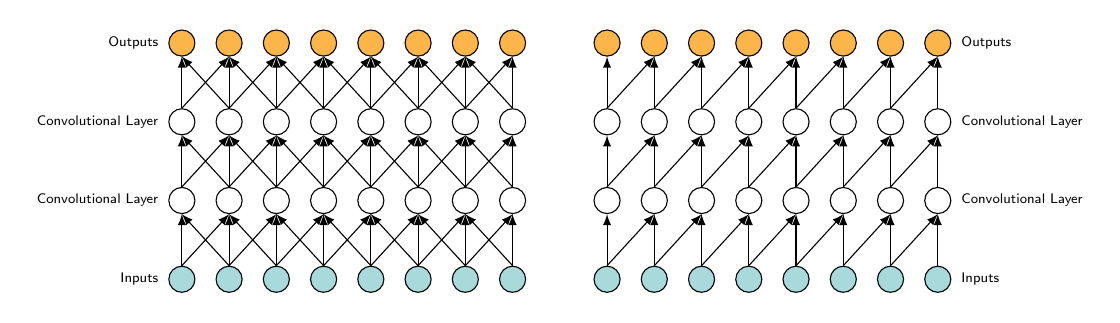
\begin{tikzpicture}[cir/.style={circle,draw=#1,minimum size=0.01cm},y=0.6cm,font=\sffamily]
\begin{scope}[rotate=90]
\foreach \x in {0,...,3} {
  \foreach \y in {0,...,7} {
    \ifnum \x=0
      \node[cir=black, fill=lightblue] (\alphalph{\x+1}\y) at (\x, \y) {};
    \else
      \ifnum \x=3
        \node[cir=black, fill=lightorange] (\alphalph{\x+1}\y) at (\x, \y) {};
      \else
        \node[cir=black] (\alphalph{\x+1}\y) at (\x, \y) {};
      \fi
    \fi
  }
}

\foreach \x in {0,...,3} {
  \foreach \y in {9,...,16} {
    \ifnum \x=0
      \node[cir=black, fill=lightblue] (\alphalph{\x+1}\y) at (\x, \y) {};
    \else
      \ifnum \x=3
        \node[cir=black, fill=lightorange] (\alphalph{\x+1}\y) at (\x, \y) {};
      \else
        \node[cir=black] (\alphalph{\x+1}\y) at (\x, \y) {};
      \fi
    \fi
  }
}

\foreach \i/\j in {a/b,b/c,c/d} {
  \foreach \cnto in {9,...,16} {
    \foreach \cntt in {9,...,16} {
      \ifnum \numexpr\cnto-1\relax=\cntt
        \draw[-latex] (\i\cnto.north) -- (\j\cntt.south);
      \fi
      \ifnum \cnto=\cntt
        \draw[-latex] (\i\cnto.north) -- (\j\cntt.south);
      \fi
      \ifnum \numexpr\cnto+1\relax=\cntt
        \draw[-latex] (\i\cnto.north) -- (\j\cntt.south);
      \fi
    }
  }
}

\foreach \i/\j in {a/b,b/c,c/d} {
  \foreach \cnto in {0,...,7} {
    \foreach \cntt in {0,...,7} {
      \ifnum \numexpr\cnto-1\relax=\cntt
        \draw[-latex] (\i\cnto.north) -- (\j\cntt.south);
      \fi
      \ifnum \cnto=\cntt
        \draw[-latex] (\i\cnto.north) -- (\j\cntt.south);
      \fi
    }
  }
}
\end{scope}

\draw (a0) node[black,right=0.5em] {\tiny Inputs};
\draw (b0) node[black,right=0.5em] {\tiny Convolutional Layer};
\draw (c0) node[black,right=0.5em] {\tiny Convolutional Layer};
\draw (d0) node[black,right=0.5em] {\tiny Outputs};

\draw (a16) node[black,left=0.5em] {\tiny Inputs};
\draw (b16) node[black,left=0.5em] {\tiny Convolutional Layer};
\draw (c16) node[black,left=0.5em] {\tiny Convolutional Layer};
\draw (d16) node[black,left=0.5em] {\tiny Outputs};

\end{tikzpicture}

\caption{Image CNN (Left) v.s. Causal CNN (Right)}\label{fig:cnn-comparison}
\end{figure}


However, CNNs are also limited by its receptive field and the fixed filters.
The fixed filters will be applied to any window of time series data, and is therefore incapable of capturing seasonal changes hidden in the data.
It is also limited by the rolling window because it is only capable of capturing the information within the receptive field.

\subsection{Recurrent Neural Networks}

Recurrent neural networks (RNNs) \citet{10.5555/65669.104451}, on the other hand, are designed for sequence modeling, and were commonly used in various natural language processing tasks.
Given the similar nature of text sequence and time series data, RNNs seem to be natural to apply to time series related tasks.
RNNs contain connections between nodes and stores a summary of the past information as a memory state.
RNNs can learn more past information because they do not have restrictions on the rolling window.
A typical RNN architecture is shown in Figure~\ref{fig:rnn}.

\begin{figure}[ht]
\centering
\begin{tikzpicture}[cir/.style={circle,draw=#1,minimum size=0.01cm},rec/.style={rectangle,draw=#1,minimum size=0.01cm},y=0.6cm,font=\sffamily]
\begin{scope}[rotate=90]
\foreach \x in {0,...,2} {
  \foreach \y in {1,...,8} {
    \ifnum \x=0
      \node[cir=black, fill=lightblue] (\alphalph{\x+1}\y) at (\x, \y) {};
    \else
      \ifnum \x=2
        \node[cir=black, fill=lightorange] (\alphalph{\x+1}\y) at (\x, \y) {};
      \else
        \node[rec=black] (\alphalph{\x+1}\y) at (\x, \y) {};
      \fi
    \fi
  }
}


\foreach \i/\j in {a/b,b/c} {
  \foreach \cnto in {1,...,8} {
    \foreach \cntt in {1,...,8} {
      \ifnum \cnto=\cntt
        \draw[-latex] (\i\cnto.north) -- (\j\cntt.south);
      \fi
    }
  }
}

% invisible node
\node[rec=black, draw=none] (b0) at (1, 0) {};
\node[rec=black, draw=none] (b9) at (1, 9) {};

% \draw[-latex] (b1.east) -- (b0.west);

\foreach \cnto in {0,...,8} {
  \foreach \cntt in {1,...,9} {
    \ifnum \numexpr\cnto+1\relax=\cntt
      \draw[-latex] (b\cntt.east) -- (b\cnto.west);
    \fi
  }
}

\end{scope}

\draw (a0) node[black,right=0.5em] {\tiny Inputs};
\draw (b0) node[black,right=0.5em] {\tiny Recurrent Layer};
\draw (c0) node[black,right=0.5em] {\tiny Outputs};

\end{tikzpicture}

\caption{Basic RNN architecture}\label{fig:rnn}
\end{figure}

For a typical RNN architecture, the hidden state $\va^{t}$ and the ouput $\vy^{t}$ at time step $t$ is in the form:
\begin{align}
        \va^{t} &= \sigma_{1} ( \mW_{a} \va^{t-1} + \mW_{x} \vx^{t} + \vb_{a} ) \\
        \vy^{y} &= \sigma_{2} ( \mW_{y} \va^{t} + \vb_{y} )
\end{align}
where $\sigma_{1}, \sigma_{2}$ are the activation functions, and $\mW_{a}, \mW_{x}, \mW_{y}, \vb_{a}, \vb_{y}$ are weights shared temporally.

However, exploding and vanishing gradients problem presist in RNNs and its variant architecture.
This problem limits the ability of RNN to store long term memory in the memory states.
With the addition of forget state in RNN variant like LSTM \citet{10.1162/neco.1997.9.8.1735}, the exploding and vanishing gradients problem can be mitigated, but it is far from completely solving the problem.
Another issue with RNNs is that the dependency between nodes makes it harder to parallelize as the computation of the current node can only be started when the previous node finishes its computation.


\section{Transformer}

With the attention machanism \citet{DBLP:journals/corr/BahdanauCB14} born to help the encoder-decoder RNN network preserving long term memory, the use of attention in various networks have become popular in recent years.
In particular, transformer model \citet{vaswani2017attention} that was introduced in 2017 is entirely built upon the self-attention machanism without the use of any recurrent architecture.
In the following subsections, we will discuss the Transformer architecture in detail.

\subsection{Positional Encoding}

In the case of natural language processing, position and order of the words are important in interpreting the language.
In recurrent neural networks, the order of the word has been naturally taken into consideration as the words are processed in a sequential manner.
However, by removing the recurrent-like architecture, Transformer itself does not have the ability to capture the position and order of each word in the sentence.
Therefore, it becomes essential to preprocess the input so that it incorporates positional information when entering the Transformer model.

Even though one can incorporate the position index into the data, it corrupts the data when the sequence is extremely long as the data at the last position will be added with a large number.
The author instead proposed to encode the position of the data in the sequence using sine and cosine functions in the form:
\begin{align}
  \begin{cases}
          \vp_{2i}^{t}   &= \sin ( w_{i} \cdot t ) \\
          \vp_{2i+1}^{t} &= \cos ( w_{i} \cdot t )
  \end{cases}
\end{align}
where
\begin{align}
        w_{i} = \frac{1}{10000^{2i/d_{\mathrm{model}}}}
\end{align}
$t$ is the position and $i$ is the feature dimension.
The benefit of such positional encoding is obvious.
For the data within the sequence length, each data will be equiped with a different encoding provided by the $\sin$ and $\cos$ functions.

\textbf{Temporal Encoding}: In time series data, positional encoding seems to be useful in capturing the temporal relationship.
However, the relative positional encoding within the sequence length limits the Transformer to only capture information in the range similar to CNNs.
\citet{haoyietal-informer-2021} proposed a method of encoding the temporal information in the input.
Specifically, it leverages the time information in the data to create the encoding.
For example, for a data point with month, day, and hour information, the temporal embedding will be a sum of the month embedding, day embedding, and hour embedding.
Each embedding is a positional encoding with fixed sequence size.
The sequence size corresponds to the finest granularity of each type of embedding.
The finest granularity of the month embedding will likely be 12 months.
The finest granularity of the day embedding will likely be 30 days.
This temporal encoding could be useful in incorporating additional temporal information in the input data.
However, it requires every data entry is associated with a time stamp, which might sometimes not be the case.


\subsection{Multi-Head Self-Attention}

The self attention machanism is the major component in the Transformer.
The attention takes the encoded input representation in the form of (query, key, value) and performs the scaled dot-product as a variant of the dot-product attention \citet{luong-etal-2015-effective}:
\begin{equation}
        \gA ( \mW, \mK, \mV ) = \mathrm{Softmax} ( \frac{\mQ \mK^{\top}}{\sqrt{d}} ) \mV
\end{equation}
where $\mQ \in \R^{L_{Q} \times d}, \mK \in \R^{L_{K} \times d}, \mV \in \R^{L_{V} \times d}$ and $d$ is the input dimension.

To further increase the expressive power of the model, multiple attention heads are used to run the self-attention machanism in parallel.
The author claims that the multi-head attention will allow the model to learn attention from different position of the input representation.
Specifically, the multi-head attention takes in the form:
\begin{equation}
\mathrm{MultiHead} ( \mQ, \mK, \mV ) = [\mathrm{head}_{1}:\ldots:\mathrm{head}_{h}] \mW^{O}
\end{equation}
where
\begin{equation}
\mathrm{head}_{i} = \gA (\mQ \mW_{i}^{Q}, \mK \mW_{i}^{K}, \mV \mW_{i}^{V} )
\end{equation}
$h$ is the number of heads, and $\mW_{i}^{Q}, \mW_{i}^{K}, \mW_{i}^{V}, \mW^{O}$ are learnable parameters.

\textbf{\textit{ProbSparse} Self-Attention}: 
A major problem in Transformer is the quadratic computation time complexity and the $O(L_{Q} L_{K})$ memory comsumption.
The self-attention machanism has potential sparsity and could be utilized to reduce the computational cost.
Previous studies \citep{child2019sparsetransformer, NEURIPS2019_6775a063, Beltagy2020Longformer} have shown multiple attempts in reducing the computational complexity by using heuristic methods to search for the sparsity of the self-attention.
In \citet{haoyietal-informer-2021}, they propose to extract the top-$u$ queries under a sparsity measurement in the form:
\begin{equation}
        M(\vq_{i}, \mK) = \ln{\underset{j=1}{\overset{L_{K}}{\sum}} e^{\frac{\vq_{i}\vk_{j}^{\top}}{\sqrt{d}}}} - \frac{1}{L_{K}} \overset{L_{K}}{\underset{j=1}{\sum}} \frac{\vq_{i} \vk_{j}^{\top}}{\sqrt{d}},
\end{equation}
The $u$ is set to be $u = c \cdot \ln{L_{Q}}$ where $c$ is a constant sampling factor.
By only utilizing the top-$u$ queries in the dot product computation, the self-attention time complexity can be reduced from quadratic time complexity to $O(\ln{L_{Q}})$.
The memory usage will also drop from $O(L_{K}L_{Q})$ to $O(L_{K}\ln{L_{Q}})$.
However, the $u = c \cdot \ln{L_{Q}}$ is not always smaller than $L_{Q}$ when $c \ge 3$.
Therefore, when $L_{Q}$ is small and $c \ge 3$, it is equivalent to the traditional self-attention mechanism.

\subsection{Encoder and Decoder}

The encoder and docoder are built upon the self-attention layer and standard techniques like layer normalization, dropout, and residual connection.
Each encoder layer typically consists of a \textbf{multi-head attention} layer, a \textbf{dropout} layer, a \textbf{residual} connection, and a \textbf{layernorm} layer.
The input of the encoder at sequence $t$ is shaped to $\mX_{en}^{t} \in \R^{L_{x} \times d_{\mathrm{model}}}$ after the positional encoding.
$L_{x}$ is the size of the rolling window up to the prediction point.
In the decoder, the input is feeded as the concatenation of the start token and the prediction sequence:
\begin{equation}
        \mX_{de}^{t} = \mathrm{Concat} ( \mX_{\mathrm{token}}^{t}, \mX_{\mO}^{t} ) \in \R^{(L_{\mathrm{token}} + L_{t}) \times d_{\mathrm{model}}}
\end{equation}
It is commonly found that utilizing a earlier slide of the sequence just before the prediction sequence would help the decoder in capturing the sequence relationship.
$\mX_{\mathrm{token}}^{t}$ would be the last $L_{\mathrm{token}}$ of the $\mX_{en}^{t}$ sequence.

In later literature \citep{devlin-etal-2019-bert, radford2019language}, an important observation is that good performance can be obtained by using only the encoder or the decoder architecture.
It is also observed in the experiment section that using encoder-decoder or decoder only architecture can lead to similar performance.

\textbf{Self-Attention Distilling}:
Inspired by dilated convolution, \citet{haoyietal-informer-2021} chose to distill their self-attention layer by performing 1D convolution and max pooling on the output.
Specifically, the output from $j$-th layer into $(j+1)$-th layer is in the form:
\begin{equation}
\mX_{j+1}^{t} = \mathrm{MaxPool} \Big( \mathrm{ELU} \big( \mathrm{Conv1d} ( {[\mX_{j}^{t}]}_{AB} ) \big) \Big)
\end{equation}
where ${[\cdot]}_{AB}$ is the output of the multi-head ProbSparse self-attention and $\mathrm{Conv1d}(\cdot)$ is an 1-D convolutional filter with kernel width 3.
The max pooling layer will downsample the output to half of the original size and thus reduce the memory usage.

\section{Experiment}

\subsection{Dataset}

In the experiment, a rather noisy dataset is chosen to test the performance of the Transformer as well established datasets have been already benchmarked in many papers.

The dataset is provided in the kaggle competition ``$\mathrm{Jane \ Street \ Market \ Prediction}$''.
A total of 130 anonymized features representing real stock market data is provided in the dataset.
Each data entry represents a trading opportunity, and the model shall predict whether to attempt a trade or not to maximize the return.
In addition to the trading features, 5 returns over different time horizons are provided to guide the model in maximizing the return.
However, only one of the return specified by the organizer will be used in evaluating the overall model performance.
Each training data is also associated with a weight to be used in evaluating the overall return.
Specifically, the evaluation is measured on a utility score with the following form:
\begin{gather}
        p_{i} = \underset{j}{\sum} (\mathrm{weight}_{i, j} \cdot \mathrm{resp}_{i, j} \cdot \mathrm{action}_{i, j} ), \\
        t = \frac{\sum p_{i}}{\sqrt{\sum p_{i}^{2}}} \cdot \sqrt{\frac{250}{|i|}}, \\
        u = \mathrm{min}(\mathrm{max}(t, 0), 6) \sum p_{i}
\end{gather}
where $p_{i}$ is the overall weighted sum of the specified return `$\mathrm{resp}$' for each date $i$, $|i|$ is the number of days available in the test dataset, and the utility score $u$ is the overall return $\sum p_{i}$ multiplying a weighted number clipped between the range $[0, 6]$.
A relative date where the trading opportunity is available is given for each training entry with a total of 500 days available in the training dataset, and a relative ordering of the training entry is also given.

\subsection{Data Analysis}

A notable characteristic of the dataset is that the time interval between adjacent trading opportunities is dynamic.
Unlike many traditional time series dataset that is recorded on a fixed time interval, the trading dataset provided by jane street is recorded anytime during the trading period.
The trading frequency for a given date can be as high as ten thousand times and as low as 22 times.

This characteristic becomes the main obstacle in training time series model like Transformer.
In image or text data, the distance between two features in the input is mostly fixed.
For image data, the neighbor pixel has a fixed length of one to a center pixel.
In text data, each pair of adjacent words has a fixed length of one as well.
Such information is implicited provided to the model as the input data being computed because adjacent data must exhibit similar characteristic.

However, in the trading prediction, only trading opportunities are given, and the adjacent set of features can likely be two distant moments that have a time interval up to a few hours or as short as one second.

\subsection{Experiment Setup}

The experiment is conducted on one 8GB RTX 2070 Super Graphics Card and AMD 3600 CPU\@.
Many different setups have been experimented.
Different number of encoder and decoder layers in the range of $[0, 4]$, prediction window size $L_{t}$ \{3, 12, 24, 48, 96, 128\}, different depth of the model $d_{\mathrm{model}}$, feed forward network $d_{\mathrm{ff}}$, the number of heads in the self attention, and the attention mechanism [prob, full] have been experimented to tune the performance of the model.
Two different loss functions are experimented in the experiment.
One metric is the binary cross entropy loss which the problem is framed to be a binary classification problem.
The action will be taken if the $\mathrm{resp}$ is greater than zero meaning that under a certain time horizon, the return is positive.
Another metric is the Smooth L1 loss or the Huber loss.
The problem in this case is framed to be a regression problem where the gold is to predict the return as close as possible with the groundtruth $\mathrm{resp}$.
Other traditional hyperparameters including learning rate, dropout rate, batch size, and early stopping patience are also experimented.

\subsection{Results and Analysis}

The main difference in performance comes from the loss function.
Framing the problem to be a binary classification problem generally will perform poorly compared to framing the it to be a regression problem.
Choosing a large $d_{\mathrm{model}}$ and $d_{\mathrm{ff}}$ can cause learning problem as well.
For example, the original architecture chose $d_{\mathrm{model}}$ and $d_{\mathrm{ff}}$ to be $512$ and $2048$ respectively.
The number of features in the dataset is only $130$, and in their dataset, the number of features is only $7$.
The wide model layer makes the feature spreading in the output and sparser than the original feature space.
The convolutional layer with receptive field of 3 can therefore only capture a small area of features and degrade the model performance by a large margin.

The default configuration is shown in Table~\ref{tab:default-conf}.
$L_{x}$ represents the input sequence length or the rolling window length of the input into the encoder.
$L_{\mathrm{token}}$ represents the rolling window length of the input to the decoder.
$L_{t}$ is the number of prediction output.
When $L_{t} > 1$, the prediction is a multistep prediction meaning that the model tries to predict multiple future consecutive events.
$L_{e}$ represents the number of the encoder layers, $L_{d}$ represents the number of the decoder layers, and $L_{h}$ represents the number of attention heads.
lr represents the learning rate, which is commonly seen in deep learning applications.

Under the default hyperparameters setting, the model can achieve a utility score of $2143.54$.
With only two layers of decoders and no encoders, the model is still able to achieve $2199.20$ which is even higher than the naive transformer model.
Based on the experiment, the encoder does not seem to contribute much to the final performance, and this result is also constantly observed in other NLP literature.
The change in $L_{\mathrm{token}}$ does not lead to high performance gain as well.
For a decoder only architecture, $L_{\mathrm{token}} = 48$ is sufficient to achieve the best performance in all tested Transformer architecture.
\textit{ProbSparse} self-attention does save tremendous amount of memory.
Under the same standard setting with default hyperparameters configuration, the batch size can be two times larger when using \textit{ProbSparse} other than the Full attention.

\begin{table}[ht]
\centering
\resizebox{\textwidth}{!}{%
\begin{tabular}{@{}cccccccccccc@{}}
\toprule
Attention & Loss  & $L_{x}$ & $L_{\mathrm{token}}$ & $L_{t}$ & $d_{\mathrm{model}}$ & $d_{\mathrm{ff}}$ & dropout & $L_{e}$ & $L_{d}$ & $L_{h}$ & lr   \\
\midrule
Full      & Huber & $96$     & $48$                & $1$     & $128$                & $128$             & $0.2$   & $1$     & $1$     & $8$     & $0.001$ \\
\bottomrule
\end{tabular}%
}
\caption{Default Hyperparameters}\label{tab:default-conf}
\end{table}

% \begin{table}[ht]
% \centering
% \resizebox{\textwidth}{!}{%
% \begin{tabular}{@{}ccccccccccccccccc@{}} \toprule
% \multirow{2}{*}{Attention} &
%   \multirow{2}{*}{Loss} &
%   \multicolumn{3}{c}{$L_{x}$/$L_{\mathrm{token}}$} &
%   \multicolumn{1}{c}{$L_{t}$} &
%   \multicolumn{3}{c}{$d_{\mathrm{model}}$/$d_{\mathrm{ff}}$} &
%   \multicolumn{2}{c}{dropout} &
%   \multicolumn{3}{c}{$L_{e}$/$L_{d}$} \\
%   \cmidrule(lr){3-5}
%   \cmidrule(lr){6-6}
%   \cmidrule(lr){7-9}
%   \cmidrule(lr){10-11}
%   \cmidrule(l){12-14}
%                             &       & 24/12   & 96/48   & 256/128 &  3      & 64/64   & 128/64  & 128/128 & 0.1 & 0.3 & 0/1 & 2/2 & 0/2 \\ \midrule
% \multirow{2}{*}{ProbSparse} & BCE   &         &         &         &         &         &         &         &     &     &     &     &     \\
%                             & Huber & 1366.66 & 2143.54 & 2002.31 & 2189.07 & 2196.33 & 2080.09 &         &     &     &     &     &     \\ \midrule
% \multirow{2}{*}{Full}       & BCE   &         &         &         &         &         &         &         &     &     &     &     &     \\
%                             & Huber &         &         &         &         &         &         &         &     &     &     &     &     \\ \bottomrule
% \end{tabular}%
% }
% \caption{Time-series Forecasting Results}\label{tab:forcasting}
% \end{table}



\section{Conclusion}

In this capstone project report, we discuss different deep learning architecture that could be applied to time series data.
We also further investigate the Transformer and its state of the art application in the times series data.
In the experiment section, we investigate the usage of Transformer in a particular noisy dataset, and pinpoint some of the drawbacks with the Transformer architecture.
It would be interesting to see further improvement in time series forecasting and more mathematically proven methods in dealing with time series data.

\bibliography{capstone_project_report}
\bibliographystyle{iclr2021_conference}

\end{document}
